\mfpicnumber{1}

\opengraphsfile{AppLines}

\setcounter{footnote}{0}

\setlength{\extrarowheight}{2pt}

\label{AppLines}
 
In Section \ref{Distance}, we concerned ourselves with the finite line segment between two points $P$ and $Q$.  Specifically, we found its length (the distance between $P$ and $Q$) and its midpoint.  In this section, our focus will be on the \textit{entire} line, and ways to describe it algebraically.  Consider the generic situation below.

\begin{center}

\begin{mfpic}[15]{0}{4}{0}{4}
\point[3pt]{(1,3), (3,1)}
\arrow \reverse \arrow \polyline{(0,4),(4,0)}
\tlabel(1.5,3){\small $P\left(x_{\mbox{\tiny$0$}}, y_{\mbox{\tiny$0$}}\right)$}
\tlabel(3.5,1){\small $Q\left(x_{\mbox{\tiny$1$}}, y_{\mbox{\tiny$1$}}\right)$}
\end{mfpic}

\end{center}

To give a sense of the `steepness' of the line, we recall that we can compute the \textbf{slope} of the line as follows. (Read the character $\Delta$ as `change in'.)

\medskip

\colorbox{ResultColor}{\bbm

%\smallskip

\begin{eqn} \label{slope} The \index{slope ! definition} \textbf{slope} $m$ of the line containing the points $P\left(x_{\mbox{\tiny$0$}}, y_{\mbox{\tiny$0$}}\right)$ and $Q\left(x_{\mbox{\tiny$1$}}, y_{\mbox{\tiny$1$}}\right)$ is: \index{line ! slope of} \index{slope ! of a line}

\[ m  = \dfrac{y_{\mbox{\tiny$1$}} - y_{\mbox{\tiny$0$}}}{x_{\mbox{\tiny$1$}} - x_{\mbox{\tiny$0$}}} = \dfrac{\Delta y}{\Delta x},\]

provided $x_{\mbox{\tiny$1$}} \neq x_{\mbox{\tiny$0$}}$, that is, $\Delta x \neq 0$.

\end{eqn}

\ebm}

\medskip

A couple of notes about Equation \ref{slope} are in order.  First, don't ask why we use the letter `$m$' to represent slope.  There are many explanations out there, but apparently no one really knows for sure.\footnote{See  \href{http://mathforum.org/dr.math/faq/faq.terms.html}{\underline{www.mathforum.org}} or \href{http://mathworld.wolfram.com/Slope.html}{\underline{www.mathworld.wolfram.com}} for discussions on this topic.} Secondly, the stipulation  $x_{\mbox{\tiny$1$}} \neq x_{\mbox{\tiny$0$}}$ (or $\Delta x \neq 0$) ensures that we aren't trying to divide by zero.  The reader is invited to pause to think about what is happening geometrically when the `change in $x$' is $0$; the anxious reader can skip along to the next example.

\begin{ex}  Find the slope of the line containing the following pairs of points, if it exists.  Plot each pair of points and the line containing them.

\begin{multicols}{2}
\begin{enumerate}

\item  $P(0,0)$, $Q(2,4)$
\item  $P(-1,2)$, $Q(3,4)$

\setcounter{HW}{\value{enumi}}
\end{enumerate}
\end{multicols}

\begin{multicols}{2}
\begin{enumerate}
\setcounter{enumi}{\value{HW}}

\item  $P(-2,3)$, $Q(2,-3)$
\item  $P(-3,2)$, $Q(4,2)$

\setcounter{HW}{\value{enumi}}
\end{enumerate}
\end{multicols}

\begin{multicols}{2}
\begin{enumerate}
\setcounter{enumi}{\value{HW}}

\item  $P(2,3)$, $Q(2,-1)$
\item  $P(2,3)$, $Q(2.1, -1)$

\end{enumerate}
\end{multicols}

{\bf Solution.}  In each of these examples, we apply the slope formula, Equation \ref{slope}.

\begin{enumerate}

\item  \begin{tabular}{m{2.5in}m{2.5in}} $ m = \dfrac{4 - 0}{2 - 0} = \dfrac{4}{2} = 2$ & 

\begin{mfpic}[15]{-1}{5}{-1}{5}
\point[3pt]{(0,0),(2,4)}
\arrow \reverse \arrow \polyline{(-0.5,-1), (2.5, 5)}
\tlabel(0.25,-0.5){\tiny $P$}
\tlabel(2,3.5){\tiny $Q$}
\axes
\tlabel[cc](5,-0.5){\scriptsize $x$}
\tlabel[cc](0.5,5){\scriptsize $y$}
\xmarks{1,2,3,4}
\ymarks{1,2,3,4}
\tlpointsep{4pt}
\axislabels {x}{{\tiny $1$} 1, {\tiny $2$} 2, {\tiny $3$} 3, {\tiny $4$} 4}
\axislabels {y}{{\tiny $1$} 1, {\tiny $2$} 2, {\tiny $3$} 3, {\tiny $4$} 4}
\end{mfpic} \\

\end{tabular}

\item \begin{tabular}{m{2.5in}m{2.5in}} $ m = \dfrac{4 - 2}{3 - (-1)} = \dfrac{2}{4} = \dfrac{1}{2}$ &

\begin{mfpic}[15]{-2}{4}{0}{5}
\point[3pt]{(-1,2),(3,4)}
\arrow \reverse \arrow \polyline{( -2,1.5), (4 ,4.5 )}
\tlabel(-1,1.5){\tiny $P$}
\tlabel(3,3.5){\tiny $Q$}
\axes
\tlabel[cc](4,-0.5){\scriptsize $x$}
\tlabel[cc](0.5,5){\scriptsize $y$}
\xmarks{-1,1,2,3}
\ymarks{1,2,3,4}
\tlpointsep{4pt}
\axislabels {x}{{\tiny $-1 \hspace{7pt}$} -1,{\tiny $1$} 1, {\tiny $2$} 2, {\tiny $3$} 3}
\axislabels {y}{{\tiny $1$} 1, {\tiny $2$} 2, {\tiny $3$} 3, {\tiny $4$} 4}
\end{mfpic} \\

\end{tabular}

\item  \begin{tabular}{m{2.5in}m{2.5in}} $ m = \dfrac{-3 - 3}{2 - (-2)} = \dfrac{-6}{4} = -\dfrac{3}{2}$ &

\begin{mfpic}[15]{-4}{4}{-5}{5}
\point[3pt]{(-2,3),(2,-3)}
\arrow \reverse \arrow \polyline{( -3,4.5), (3 ,-4.5 )}
\tlabel(-1.5,3){\tiny $P$}
\tlabel(2.5,-3){\tiny $Q$}
\axes
\tlabel[cc](4,-0.5){\scriptsize $x$}
\tlabel[cc](0.5,5){\scriptsize $y$}
\xmarks{-3,-2,-1,1,2,3}
\ymarks{-4,-3,-2,-1,1,2,3,4}
\tlpointsep{4pt}
\axislabels {x}{{\tiny $-3 \hspace{7pt}$} -3,{\tiny $-2 \hspace{7pt}$} -2,{\tiny $-1 \hspace{7pt}$} -1,{\tiny $1$} 1, {\tiny $2$} 2, {\tiny $3$} 3}
\axislabels {y}{{\tiny $-4$} -4, {\tiny $-3$} -3, {\tiny $-2$} -2, {\tiny $-1$} -1,{\tiny $1$} 1, {\tiny $2$} 2, {\tiny $3$} 3, {\tiny $4$} 4}
\end{mfpic} \\

\end{tabular}

\item  \begin{tabular}{m{2.5in}m{2.5in}} $ m = \dfrac{2 - 2}{4 - (-3)} = \dfrac{0}{7} = 0$ &

\begin{mfpic}[15]{-5}{5}{0}{4}
\point[3pt]{(-3,2),(4,2)}
\arrow \reverse \arrow \polyline{( -5,2), (5,2)}
\tlabel[cc](-3,1.5){\tiny $P$}
\tlabel[cc](4,1.5){\tiny $Q$}
\axes
\tlabel[cc](5,-0.5){\scriptsize $x$}
\tlabel[cc](0.5,4){\scriptsize $y$}
\xmarks{-4,-3,-2,-1,1,2,3,4}
\ymarks{1,2,3}
\tlpointsep{4pt}
\axislabels {x}{{\tiny $-4 \hspace{7pt}$} -4,{\tiny $-3 \hspace{7pt}$} -3,{\tiny $-2 \hspace{7pt}$} -2,{\tiny $-1 \hspace{7pt}$} -1,{\tiny $1$} 1, {\tiny $2$} 2, {\tiny $3$} 3, {\tiny $4$} 4}
\axislabels {y}{{\tiny $1$} 1, {\tiny $2$} 2, {\tiny $3$} 3}
\end{mfpic} \\

\end{tabular}

\item  \begin{tabular}{m{3in}m{2in}} $ m = \dfrac{-1 - 3}{2 - 2} = \dfrac{-4}{0}$, which is undefined &

\begin{mfpic}[15]{0}{3}{-4}{4}
\point[3pt]{(2,3),(2,-1)}
\arrow \reverse \arrow \polyline{( 2,-4), (2,4)}
\tlabel[t](2.25,3){\tiny $P$}
\tlabel[t](2.25,-1){\tiny $Q$}
\axes
\tlabel[cc](3,-0.5){\scriptsize $x$}
\tlabel[cc](0.5,4){\scriptsize $y$}
\xmarks{1,2}
\ymarks{-3,-2,-1,1,2,3}
\tlpointsep{4pt}
\axislabels {x}{{\tiny $1$} 1, {\tiny $2$} 2}
\axislabels {y}{{\tiny $-3$} -3, {\tiny $-2$} -2, {\tiny $-1$} -1,{\tiny $1$} 1, {\tiny $2$} 2, {\tiny $3$} 3}
\end{mfpic} \\

\end{tabular}

\item  \begin{tabular}{m{3in}m{2in}} $ m = \dfrac{-1 - 3}{2.1 - 2} = \dfrac{-4}{0.1}=-40$ &

\begin{mfpic}[15]{0}{3}{-4}{4}
\point[3pt]{(2,3),(2.1,-1)}
\arrow \reverse \arrow \polyline{( 1.99,3.4), (2.15,-3)}
\tlabel[t](2.25,3){\tiny $P$}
\tlabel[t](2.25,-1){\tiny $Q$}
\axes
\tlabel[cc](3,-0.5){\scriptsize $x$}
\tlabel[cc](0.5,4){\scriptsize $y$}
\xmarks{1,2}
\ymarks{-3,-2,-1,1,2,3}
\tlpointsep{4pt}
\axislabels {x}{{\tiny $1$} 1, {\tiny $2$} 2}
\axislabels {y}{{\tiny $-3$} -3, {\tiny $-2$} -2, {\tiny $-1$} -1,{\tiny $1$} 1, {\tiny $2$} 2, {\tiny $3$} 3}
\end{mfpic} \\

\end{tabular}

\end{enumerate}

\label{slopeex}

\vspace{-.2in}

\qed

\end{ex} 

\smallskip

A few comments about Example \ref{slopeex} are in order.  First, if the slope is positive then the resulting line is said to be `increasing', meaning as we move from left to right,\footnote{That is, as we increase the $x$-values \ldots} the $y$-values are getting larger.\footnote{We'll have more to say about this idea in Section \ref{ConstantandLinearFunctions}.}  Similarly, if the slope is negative, we say the line is `decreasing', since as we move from left to right, the $y$-values are getting smaller.  A slope of $0$ results in a horizontal line which we say is `constant', since the $y$-values here remain unchanged as we move from left to right,  and an undefined slope results in a vertical line.\footnote{Some authors use the unfortunate moniker `no slope' when a slope is undefined.  It's easy to confuse the notions of `no slope' with `slope of $0$'.  For this reason, we will describe slopes of vertical lines as `undefined'.}   

\medskip

Second, the larger the slope is in absolute value, the steeper the line.  You may recall from Intermediate Algebra that slope can be described as the ratio `$\frac{\mbox{\small rise}}{\mbox{\small run}}$'.  For example, if the slope works out to be $\frac{1}{2}$, we can interpret this as a `rise' of $1$ unit upward for every `run' of $2$ units to the right:

\begin{center}

\begin{mfpic}[20]{-2}{4}{0}{5}
\point[3pt]{(-1,2),(1,3), (3,4)}
\arrow \reverse \arrow \polyline{( -2,1.5), (4 ,4.5 )}
\dashed \polyline{(-1,2), (1,2), (1,3), (3,3), (3,4)}
\tlabel[cc](2,2.5){\tiny `over $2$'}
\tlabel[t](3.25,3.5){\tiny `up $1$'}
\axes
\tlabel[cc](4,-0.5){\scriptsize $x$}
\tlabel[cc](0.5,5){\scriptsize $y$}
\xmarks{-1,1,2,3}
\ymarks{1,2,3,4}
\tlpointsep{4pt}
\axislabels {x}{{\tiny $-1 \hspace{7pt}$} -1,{\tiny $1$} 1, {\tiny $2$} 2, {\tiny $3$} 3}
\axislabels {y}{{\tiny $1$} 1, {\tiny $2$} 2, {\tiny $3$} 3, {\tiny $4$} 4}
\end{mfpic}

\end{center}


In this way, we may view the slope as  `the \textbf{rate of change} of $y$ with respect to $x$'.  From the expression \[ m = \dfrac{\Delta y}{\Delta x}\] we get $\Delta y = m \Delta x$ so that the $y$-values change `$m$' times as fast as the $x$-values.  We'll have more to say about this concept in Section \ref{ConstantandLinearFunctions} when we explore applications of linear functions;  presently, we will keep our attention focused on the analytic geometry of lines.  To that end, our next task is to find algebraic equations that describe lines and we start with a discussion of vertical and horizontal lines.

\pagebreak

Consider the two lines shown below: $V$ (for `V'ertical Line) and $H$ (for `H'orizontal Line).    

\smallskip

\hspace{1in} \begin{tabular}{m{2in}m{3in}}

\begin{mfpic}[18]{-1}{5}{-5}{5}
\arrow \reverse \arrow \polyline{(3,-5), (3,5)}
\axes
\tlabel[cc](5,-0.5){\scriptsize $x$}
\tlabel[cc](0.5,5){\scriptsize $y$}
\xmarks{1,2,3,4}
\ymarks{-4,-3,-2,-1,1,2,3,4}
\tlpointsep{5pt}
\scriptsize
\axislabels {x}{{$1$} 1, {$2$} 2, {$3$} 3, {$4$} 4}
\axislabels {y}{{$-4$} -4,{$-3$} -3,{$-2$} -2, {$-1$} -1, {$1$} 1, {$2$} 2, {$3$} 3, {$4$} 4}
\normalsize
\tcaption{The line $V$}
\end{mfpic} &
\begin{mfpic}[18]{-5}{5}{-5}{1}
\arrow \reverse \arrow \polyline{(-5,-2), (5,-2)}
\axes
\tlabel[cc](5,-0.5){\scriptsize $x$}
\tlabel[cc](0.5,1){\scriptsize $y$}
\xmarks{-4,-3,-2,-1,1,2,3,4}
\ymarks{-4,-3,-2,-1}
\tlpointsep{5pt}
\scriptsize
\axislabels {x}{{$-4 \hspace{7pt}$} -4, {$-3 \hspace{7pt}$} -3, {$-2 \hspace{7pt}$} -2, {$-1 \hspace{7pt}$} -1, {$1$} 1, {$2$} 2, {$3$} 3, {$4$} 4}
\axislabels {y}{{$-4$} -4, {$-3$} -3, {$-2$} -2, {$-1$} -1}
\normalsize
\tcaption{The line $H$}
\end{mfpic} \\

\end{tabular}

\smallskip

All of the points on the line $V$ have an $x$-coordinate of $3$.  Conversely, any point with an $x$-coordinate of $3$ lies on the line $V$.  Said differently, the point $(x,y)$ lies on $V$ if and only if $x = 3$.  Because of this, we say the equation $x=3$ \textit{describes} the line $V$, or, said differently, the \textit{graph} of the equation $x=3$ is the line $V$.  

\medskip

In Section \ref{Relations}, we'll spend a great deal of time talking about graphing equations.  For now, it suffices to know that a graph of an equation is a plot of all of the points which make the equation true.  So to graph $x=3$,  we plot all of the points $(x,y)$ which satisfy $x = 3$ and this gives us our vertical line $V$.      

\medskip

Turning our attention to $H$, we note that every point on $H$ has a $y$-coordinate of $-2$, and vice-versa.  Hence the equation $y = -2$ describes the line $H$, or the graph of the equation $y=-2$ is $H$.  In general:

\medskip

\colorbox{ResultColor}{\bbm

\begin{eqn} \label{verticalhorizontallines} Equations of Vertical and Horizontal Lines

\begin{itemize}

\item The graph of the equation $x = a$ in the $xy$-plane is a \textbf{vertical line} through $(a, 0)$.\index{line ! vertical} \index{vertical line}

\item The graph of the equation $y = b$ in the $xy$-plane is a \textbf{horizontal line} through $(0, b)$.\index{line ! horizontal} \index{horizontal line}

\end{itemize}

\end{eqn}

\ebm}

\medskip

Of course, we may be working on axes which aren't labeled with the `usual' $x$'s and $y$'s.  In this case, we understand Equation \ref{verticalhorizontallines} to say `$\text{horizontal axis label} = a$' describes a \textit{vertical} line through $(a,0)$ and  `$\text{vertical axis label} = b$' describes a \textit{horizontal} line through $(0,b)$.  


\begin{ex}  \label{horizontalverticallineex}  $~$

\begin{enumerate}  \item Graph the following equations in the $xy$-plane: 

\begin{multicols}{2}
\begin{enumerate}

\item $y = 3$ 

\item $x=-117$

\end{enumerate}
\end{multicols}

\enlargethispage{.1in}

\pagebreak

\item Find the equation of each of the given lines.

\medskip

\hspace{0.5in} \begin{tabular}{m{2.5in}m{3in}}

\begin{mfpic}[18]{-1}{5}{-5}{5}
\arrow \reverse \arrow \polyline{(2,-5), (2,5)}
\axes
\tlabel[cc](5,-0.5){\scriptsize $x$}
\tlabel[cc](0.5,5){\scriptsize $y$}
\xmarks{1,2,3,4}
\ymarks{-4,-3,-2,-1,1,2,3,4}
\tlpointsep{5pt}
\scriptsize
\axislabels {x}{{$1$} 1, {$2$} 2, {$3$} 3, {$4$} 4}
\axislabels {y}{{$-4$} -4,{$-3$} -3,{$-2$} -2, {$-1$} -1, {$1$} 1, {$2$} 2, {$3$} 3, {$4$} 4}
\normalsize
\tcaption{Line $L_{1}$}
\end{mfpic} &
\begin{mfpic}[18]{-5}{5}{-1}{5}
\arrow \reverse \arrow \polyline{(-5,3), (5,3)}
\axes
\tlabel[cc](5,-0.5){\scriptsize $t$}
\tlabel[cc](0.5,5){\scriptsize $s$}
\xmarks{-4,-3,-2,-1,1,2,3,4}
\ymarks{1,2,3,4}
\tlpointsep{5pt}
\scriptsize
\axislabels {x}{{$-4 \hspace{7pt}$} -4, {$-3 \hspace{7pt}$} -3, {$-2 \hspace{7pt}$} -2, {$-1 \hspace{7pt}$} -1, {$1$} 1, {$2$} 2, {$3$} 3, {$4$} 4}
\axislabels {y}{{$4$} 4, {$3$} 3, {$2$} 2, {$1$} 1}
\normalsize
\tcaption{Line $L_{2}$}
\end{mfpic} \\

\end{tabular}

\end{enumerate}

{\bf Solution.}

\begin{enumerate}

\item  Since we're in the familiar $xy$-plane, the graph of $y=3$ is a horizontal line through $(0,3)$, shown below on the left and the graph of $x = -117$ is a vertical line through $(-117, 0)$.  We scale the $x$-axis differently than the $y$-axis to produce the graph below on the right.

\bigskip

\begin{tabular}{m{3in}m{2.5in}}
\begin{mfpic}[18]{-5}{5}{-1}{5}
\arrow \reverse \arrow \polyline{(-5,3), (5,3)}
\axes
\tlabel[cc](5,-0.5){\scriptsize $x$}
\tlabel[cc](0.5,5){\scriptsize $y$}
\xmarks{-4,-3,-2,-1,1,2,3,4}
\ymarks{1,2,3,4}
\point[3pt]{(0,3)}
\tlabel[cc](0.75, 3.5){\scriptsize $(0,3)$}
\tlpointsep{5pt}
\scriptsize
\axislabels {x}{{$-4 \hspace{7pt}$} -4, {$-3 \hspace{7pt}$} -3, {$-2 \hspace{7pt}$} -2, {$-1 \hspace{7pt}$} -1, {$1$} 1, {$2$} 2, {$3$} 3, {$4$} 4}
\axislabels {y}{{$4$} 4,{$3$} 3, {$2$} 2, {$1$} 1}
\normalsize
\tcaption{The line $y = 3$}
\end{mfpic} &

\hspace{.3in} \begin{mfpic}[18]{-5}{1}{-5}{5}
\arrow \reverse \arrow \polyline{(-3,-5), (-3,5)}
\axes
\tlabel[cc](1,-0.5){\scriptsize $x$}
\tlabel[cc](0.5,5){\scriptsize $y$}
\point[3pt]{(-3,0)}
\tlabel[cc](-1.75, 0.5){\scriptsize $(-117,0)$}
\ymarks{-4,-3,-2,-1,1,2,3,4}
\tlpointsep{5pt}
\scriptsize
\axislabels {x}{{$-117 \hspace{10pt}$} -3}
\axislabels {y}{{$-4$} -4,{$-3$} -3,{$-2$} -2, {$-1$} -1, {$1$} 1, {$2$} 2, {$3$} 3, {$4$} 4}
\normalsize
\tcaption{The line $x=-117$}
\end{mfpic} \\

\end{tabular}

\item  Since $L_{1}$ is a vertical line through $(2,0)$, and the horizontal axis is labeled with `$x$', the equation of $L_{1}$ is $x = 2$.  Since $L_{2}$ is a horizontal line through $(0,3)$ and the vertical axis is labeled as `$s$', the equation of this line is $s = 3$.  \qed

\end{enumerate}

\end{ex}
 
\pagebreak

Using the concept of slope, we can develop equations for the other varieties of lines.  Suppose a line has a slope of $m$ and contains the point $\left(x_{\mbox{\tiny$0$}}, y_{\mbox{\tiny$0$}}\right)$.  Suppose $(x,y)$ is another point on the line, as indicated below.

\begin{center}

\begin{mfpic}[15]{-2}{4}{0}{5}
\point[3pt]{(-1,2), (3,4)}
\arrow \reverse \arrow \polyline{( -2,1.5), (4 ,4.5 )}
\dashed \polyline{(-1,2), (3,2), (3,4)}
\tlabel[t](-1.5,1.5){$\left(x_{\mbox{\tiny$0$}}, y_{\mbox{\tiny$0$}}\right)$}
\tlabel[t](3.5,4){$\left(x, y \right)$}
\end{mfpic}

\end{center}

\vspace{-.1in}

Equation \ref{slope} yields

\vspace{-.1in}

\setlength{\extrarowheight}{2pt}

\[ \begin{array}{rclr}  
                      m & = & \dfrac{y - y_{\mbox{\tiny$0$}}}{x-x_{\mbox{\tiny$0$}}} & \\
m\left(x - x_{\mbox{\tiny$0$}}\right) & = & y - y_{\mbox{\tiny$0$}} & \\ 
              y - y_{\mbox{\tiny$0$}} & = & m\left(x - x_{\mbox{\tiny$0$}}\right) & \\
   \end{array} \]

which is known as the \textbf{point-slope form} of a line.

\medskip

\colorbox{ResultColor}{\bbm

\begin{eqn} \label{pointslope} The\index{point-slope form of a line}\index{line ! point-slope form} \textbf{point-slope form} of the line with slope $m$ containing the point $\left(x_{\mbox{\tiny$0$}}, y_{\mbox{\tiny$0$}}\right)$ is the equation \[y - y_{\mbox{\tiny$0$}}  =  m\left(x - x_{\mbox{\tiny$0$}}\right)\] $ $ \vspace{-.2in}
\end{eqn}

\ebm}

\medskip

A few remarks about Equation \ref{pointslope} are in order. First, note that if the slope $m = 0$, then the line is horizontal and Equation \ref{pointslope} reduces to  $y - y_{\mbox{\tiny$0$}} = 0$ or $y = y_{\mbox{\tiny$0$}}$, as prescribed by Equation \ref{verticalhorizontallines}.\footnote{Here we have $y_{\mbox{\tiny$0$}}$ as the constant whereas in the Equation we used the letter $b$. The form $y =$ constant is what matters.} Second, we may need to change the letters in Equation \ref{pointslope} from `$x$' and `$y$' depending on the context, so while  Equation \ref{pointslope} should be committed to memory, it should be understood that `$x$' refers to whichever variable is used to label the horizontal axis, and $y$ refers to whichever variable is used to label the vertical axis. Lastly, while Equation \ref{pointslope} is, by far, the easiest way to \textit{construct} the equation of a line given a point and a slope, more often than not, the equation is solved for $y$ and simplified into the form below.

\medskip

\colorbox{ResultColor}{\bbm

\begin{eqn} \label{slopeintercept} The\index{slope-intercept form of a line}\index{line ! slope-intercept form} \textbf{slope-intercept form} of the line with slope $m$ and $y$-intercept $(0,b)$ is the equation \[y  =  mx + b\] $ $ \vspace{-.2in}
\end{eqn}

\ebm}

\smallskip

Equation \ref{slopeintercept} is probably\footnote{Hopefully?} a familiar sight from Intermediate Algebra.  You may recall from that class that the  `intercept' in `slope-intercept' comes from the fact that this line `intercepts' or crosses the $y$-axis at the point $(0,b)$.\footnote{We can verify this algebraically by setting $x=0$ in the equation $y=mx+b$ and obtaining $y = b$.} If we set the slope, $m = 0$, we obtain $y=b$, the formula for Horizontal Lines first introduced in Equation \ref{verticalhorizontallines}.  Hence, any line which has a defined slope $m$ can be represented in both point-slope and slope-intercept forms.  The only exceptions are vertical lines.\footnote{We'll have more to say about this in Section \ref{ConstantandLinearFunctions}.}  There is one equation - the aptly named 'general form' - which describes every type of line and it is presented on the next page.

\pagebreak

\colorbox{ResultColor}{\bbm

\begin{eqn} \label{generallineform} Every line may be represented by an equation of the form $Ax + By = C$, where $A$, $B$ and $C$ are real numbers for which $A$ and $B$ aren't both zero.  This is called \textit{a}  \index{line ! general form}\textbf{general form} of the line. \index{general form of a line}
\end{eqn}

\ebm}

\medskip

Note the indefinite article `a' in Equation \ref{generallineform}.  The line $y = 5$ is a general form for the horizontal line through $(0,5)$, but so are $3y = 15$ and $0.5 y = 2.5$.  The reader is left to ponder the use of the definite article `the' in Equations \ref{pointslope} and \ref{slopeintercept}.  Regardless of \textit{which} form the equation of a line takes, note that the variables involved are all raised to the first power.\footnote{Recall, $x = x^{1}$, $y = y^{1}$, etc.}  For instance, there are no $\sqrt{x}$ terms, no $y^2$ terms or any variables appearing in denominators.  Let's look at a few examples.

\begin{ex}  $~$

\begin{enumerate}

\item Graph the following equations in the $xy$-plane:

\begin{multicols}{2}
\begin{enumerate}

\item  $y = 3x - 1$

\item  $2x + 4y = 3$

\end{enumerate}
\end{multicols}

\item  Find the slope-intercept form of the line containing the points $(-1,3)$ and $(2,1)$.

\item  Find the slope-intercept form of the equation of the line below:

\begin{center}
\begin{mfpic}[15]{-1}{6}{-1}{6}
\arrow \reverse \arrow \polyline{(-1,6), (6,-1)}
\point[3pt]{(0,5),(5,0)}
\axes
\tlabel[cc](6,-0.5){\scriptsize $t$}
\tlabel[cc](0.5,6){\scriptsize $s$}
\xmarks{1,2,3,4,5}
\ymarks{1,2,3,4,5}
\tlpointsep{4pt}
\axislabels {x}{{\tiny $1$} 1, {\tiny $2$} 2, {\tiny $3$} 3, {\tiny $4$} 4, {\tiny $5$} 5}
\axislabels {y}{{\tiny $1$} 1, {\tiny $2$} 2, {\tiny $3$} 3, {\tiny $4$} 4, {\tiny $5$} 5}

\end{mfpic}


\end{center}

\end{enumerate}

\smallskip

{\bf Solution.}  

\begin{enumerate}

\item To graph a line, we need just two points on that line.  There are several ways to do this, and we showcase two of them here.  For the first equation, we recognize that $y = 3x-1$ is in slope-intercept form, $y = mx+b$, with $m = 3$ and $b = -1$.  This immediately gives us one point on the graph -- the $y$-intercept $(0,-1)$. From here, we use the slope $m = 3 = \frac{3}{1}$ and move one unit to the right and three units up, to obtain a second point on the line, $(1,2)$.  Connecting these points gives us the graph on the left at the top of the next page.  

\smallskip

The second equation,  $2x+4y = 3$, is a general form of a line.  To get two points here, we choose `convenient' values for one of the variables, and solve for the other variable.  Choosing $x=0$, for example, reduces $2x+4y = 3$ to $4y = 3$, or $y = \frac{3}{4}$.  This means the point $\left(0, \frac{3}{4} \right)$ is on the graph.  Choosing $y = 0$ gives $2x = 3$, or $x = \frac{3}{2}$.  This gives is a second point on the line, $\left(\frac{3}{2}, 0 \right)$.\footnote{You may recall, that this is the $x$-intercept of the line.} Our graph of $2x+4y = 3$ is on the right at the top of the next page.

\pagebreak 

\hspace{1in} \begin{tabular}{m{2in}m{3in}} 

\begin{mfpic}[10]{-3}{3}{-5}{5}
\point[3pt]{(0,-1), (1,2)}
\arrow \reverse \arrow \polyline{( -1,-4), (2,5)}
\axes
\tlabel[cc](3,-0.5){\scriptsize $x$}
\tlabel[cc](0.5,5){\scriptsize $y$}
\xmarks{-2,-1,1,2}
\ymarks{-4,-3,-2,-1,1,2,3,4}
\tcaption{$y = 3x-1$}
\tlpointsep{4pt}
\axislabels {x}{ {\tiny $-2 \hspace{7pt}$} -2, {\tiny $-1 \hspace{7pt}$} -1, {\tiny $1$} 1, {\tiny $2$} 2}
\axislabels {y}{{\tiny $-1$} -1, {\tiny $1$} 1, {\tiny $2$} 2, {\tiny $3$} 3, {\tiny $4$} 4}
\end{mfpic} & 

\begin{mfpic}[15]{-4}{4}{-1}{3}
\point[3pt]{( 0,0.75), (1.5,0)}
\arrow \reverse \arrow \polyline{(-3,2.25),(3,-0.75)}
\axes
\tlabel[cc](4,-0.5){\scriptsize $x$}
\tlabel[cc](0.5,3){\scriptsize $y$}
\xmarks{-3,-2,-1,1,2,3}
\ymarks{1}
\tcaption{$2x+4y = 3$}
\tlpointsep{4pt}
\axislabels {x}{ {\tiny $-3 \hspace{7pt}$} -3, {\tiny $-2 \hspace{7pt}$} -2,{\tiny $-1 \hspace{7pt}$} -1, {\tiny $1$} 1, {\tiny $2$} 2 , {\tiny $3$} 3}
\axislabels {y}{{\tiny $1$} 1,{\tiny $2$} 2}
\end{mfpic} \\

\end{tabular}

\item We'll assume we're using the familiar $(x,y)$ axis labels and begin by finding the slope of the line using Equation \ref{slope}:  $m = \frac{\Delta y}{\Delta x} = \frac{1 - 3}{2 - (-1)} = -\frac{2}{3}$.  Next, we substitute this result, along with one of the given points, into the point-slope equation of the line, Equation \ref{pointslope}. We have two options for the point $\left(x_{\mbox{\tiny$0$}}, y_{\mbox{\tiny$0$}}\right)$. We'll use $(-1,3)$ and leave it to the reader to check that using $(2,1)$ results in the same equation.  Substituting into the point-slope form of the line, we get 

\vspace{-.1in}

\setlength{\extrarowheight}{10pt}
\[\begin{array}{rclr} 
y - y_{\mbox{\tiny$0$}} & = & m\left(x - x_{\mbox{\tiny$0$}}\right)  & \\
y - 3 & = & -\dfrac{2}{3} \left(x - (-1)\right) & \\
y - 3 & = & -\dfrac{2}{3} \left(x +1 \right) & \\
y - 3& = & -\dfrac{2}{3}x - \dfrac{2}{3}\\
y& = & -\dfrac{2}{3}x - \dfrac{2}{3} + 3\\
y & = & -\dfrac{2}{3} x + \dfrac{7}{3}. \\ 
\end{array} \]

\setlength{\extrarowheight}{2pt}

We can check our answer by showing that both $(-1,3)$ and $(2,1)$ are on the graph of $y  =  -\frac{2}{3} x + \frac{7}{3}$ algebraically by showing that the equation holds true when we substitute $x = -1$ and $y=3$ and when $x = 2$ and $y = 1$.

\item  From the graph, we see that the points $(0,5)$ and $(5,0)$ are on the line, so we may proceed as we did in the previous problem.  Here, however,  we use `$t$' in place of `$x$' and `$s$' in place of `$y$' in accordance to the axis labels given.  We find the slope $m = \frac{\Delta s}{\Delta t} = \frac{0 - 5}{5 - 0} = -1$.  As before, we have two points to choose from to substitute into the point-slope formula, and, as before, we'll select one of them, $(0,5)$ and leave the computations with $(5,0)$ to the reader.  

\[\begin{array}{rclr} 
s - s_{\mbox{\tiny$0$}} & = & m\left(t - t_{\mbox{\tiny$0$}}\right)  & \\
s - 5 & = & (-1) \left(t -0 \right) & \\
s- 5 & = &-t & \\
s& = & -t + 5.\\
\end{array} \]

\enlargethispage{.1in}

As before we can check this line contains both points $(t,s) = (0,5)$ and $(t,s) = (5,0)$ algebraically.  \qed

\end{enumerate}

\end{ex}

While every point on a line holds value and meaning,\footnote{Lines missing points  - even one - usually belie some algebraic pathology which we'll discuss in more detail in Chapter \ref{RationalFunctions}.} we've reminded you of certain points, called `intercepts,' which hold special enough significance to be singled out. Formally, we define these as follows.

\medskip

\colorbox{ResultColor}{\bbm

%\smallskip

\begin{defn}  Given a graph of an equation in the $xy$-plane:

\label{interceptsdefn}

\begin{itemize}

\item  A point on a graph which is also on the $x$-axis is called an \index{$x$-intercept} \textbf{\boldmath $x$-intercept} of the graph.  To determine the $x$-intercept(s) of a graph, set $y = 0$ in the equation and solve for $x$.

\textbf{NOTE:}  $x$-intercepts always have the form:  $(x_{\mbox{\tiny$0$}},0)$.

\item  A point on a graph which is also on the $y$-axis is called an \index{$y$-intercept} \textbf{\boldmath $y$-intercept} of the graph. To determine the $y$-intercept(s) of a graph, set $x = 0$ in the equation and solve for $y$.

\textbf{NOTE:}  $y$-intercepts always have the form:  $(0,y_{\mbox{\tiny$0$}})$.

\end{itemize}

\end{defn}

\ebm}

\medskip

As usual, the labels of the axes in the problem will dictate the labels on the intercepts.  If we're working in the $vw$-plane, for instance, there would be $v$- and $w$-intercepts.

\smallskip

The last little bit of analytic geometry we need to review about lines are the concepts of `parallel' and `perpendicular' lines.  Parallel lines do not intersect,\footnote{Well, at least in Euclidean Geometry \dots} and hence, parallel lines necessarily have the same slope.  Perpendicular lines intersect at a right ($90^{\circ}$) angle.   The relationship between these slopes is somewhat more complicated, and is summarized below.

\medskip

\colorbox{ResultColor}{\bbm

%\smallskip

\begin{thm}  Suppose line $L_{\mbox{\tiny$1$}}$ has slope $m_{\mbox{\tiny$1$}}$ and line $L_{\mbox{\tiny$2$}}$ has slope $m_{\mbox{\tiny$2$}}$:


\label{parallelperpendicularslopetheorem}


\begin{itemize}

\item $L_{\mbox{\tiny$1$}}$ and $L_{\mbox{\tiny$2$}}$ are parallel (written $L_{\mbox{\tiny$1$}} \parallel L_{\mbox{\tiny$2$}}$) if and only if $m_{\mbox{\tiny$1$}} = m_{\mbox{\tiny$2$}}$.

\item If $m_{\mbox{\tiny$1$}} \neq 0$ and  $m_{\mbox{\tiny$2$}} \neq 0$ then $L_{\mbox{\tiny$1$}}$ and $L_{\mbox{\tiny$2$}}$ are perpendicular (written $L_{\mbox{\tiny$1$}} \perp L_{\mbox{\tiny$2$}}$) if and only if $m_{\mbox{\tiny$1$}} m_{\mbox{\tiny$2$}} = -1$.

\textbf{NOTE:} $m_{\mbox{\tiny$1$}} m_{\mbox{\tiny$2$}} = -1$  is equivalent to $m_{\mbox{\tiny$2$}} = -\dfrac{1}{m_{\mbox{\tiny$1$}}}$, so that perpendicular lines have slopes which are `opposite reciprocals' of one another.

\end{itemize}

\end{thm}

\ebm}

\begin{center}

\begin{tabular}{cc}

\begin{mfpic}[15]{-1}{5}{-1}{5}
\tlabel[cc](5,-0.5){\scriptsize $x$}
\tlabel[cc](0.5,5){\scriptsize $y$}
\tlabel[cc](4.5,4){\scriptsize $L_{\mbox{\tiny$1$}}$}
\tlabel[cc](3.5,5){\scriptsize $L_{\mbox{\tiny$2$}}$}
\arrow \reverse \arrow \polyline{(-1,-1), (4,4)}
\arrow \reverse \arrow \polyline{(-2,0), (3,5)} 
\tlpointsep{4pt}
\tcaption{$L_{\mbox{\tiny$1$}} \parallel L_{\mbox{\tiny$2$}}$, $m_{\mbox{\tiny$1$}} = m_{\mbox{\tiny$2$}}$}
\axes

\end{mfpic} \hspace{1.5in} & 

\begin{mfpic}[15]{-1}{5}{-1}{5}
\tlabel[cc](5,-0.5){\scriptsize $x$}
\tlabel[cc](0.5,5){\scriptsize $y$}
\tlabel[cc](4.5,4){\scriptsize $L_{\mbox{\tiny$1$}}$}
\tlabel[cc](5,-1){\scriptsize $L_{\mbox{\tiny$2$}}$}
\arrow \reverse \arrow \polyline{(-1,-1), (4,4)}
\arrow \reverse \arrow \polyline{(-1,5), (4.5,-0.5)}
\polyline{(2,2), (1.75, 2.25), (2,2.5), (2.25, 2.25)} 
\point[3pt]{(2,2)}
\tlpointsep{4pt}
\axes
\tcaption{$L_{\mbox{\tiny$1$}} \perp L_{\mbox{\tiny$2$}}$, $m_{\mbox{\tiny$1$}} m_{\mbox{\tiny$2$}} = -1$}

\end{mfpic} \\


\end{tabular}

\end{center}


A few remarks about Theorem \ref{parallelperpendicularslopetheorem} are in order.  First off, the theorem assumes that the slopes of the lines exist.  The reader is encouraged to think about the case when one (or both) of the slopes don't exist.  Along those same lines, the reader is encouraged to think about why the stipulations $m_{\mbox{\tiny$1$}} \neq 0$ and $m_{\mbox{\tiny$2$}} \neq 0$ appear in the statement regarding slopes of perpendicular lines, and what happens in this case as well.  (Think geometrically!)   In Exercise \ref{perpendicularlineproof}, you'll prove the assertion about the slopes of perpendicular lines.  For now, we accept it as true and use it in the following example.

\begin{ex}  For line $y = 2x-1$ and the point $(3,4)$, find:

\begin{enumerate}

\item the equation of the line parallel to the given line which contains the given point.

\item   the equation of the line perpendicular to the given line which contains the given point.  Check your answers by graphing them, along with the original line, using a graphing utility.

\end{enumerate}

{\bf Solution.}

\begin{enumerate}

\item Since $y = 2x-1$ is already in slope-intercept form, we have the slope $m = 2$.  To find the line parallel to this line containing $(3,4)$, we use the point-slope form with $m = 2$ to get: \[\begin{array}{rclr} 
y - y_{\mbox{\tiny$0$}} & = & m\left(x - x_{\mbox{\tiny$0$}}\right)  & \\
y - 4 & = & 2 \left(x - 3\right) & \\
y - 4 & = & 2x - 6 & \\
y& = & 2x-2\\
\end{array} \] Algebraically, we can verify that the slope is indeed $2$ and that when $x =3$ we get $y = 4$.  Using a graphing utility with a window centered at the point $(3, 4)$,  we graph both $y = 2x-1$ and $y = 2x-2$ below on the left and observe that they appear to be parallel.

\item To find the line perpendicular to $y = 2x-1$ containing $(3,4)$, we use the slope $m = -\frac{1}{2}$ in the point-slope formula:\[\begin{array}{rclr} 
y - y_{\mbox{\tiny$0$}} & = & m\left(x - x_{\mbox{\tiny$0$}}\right)  & \\ [3pt]
y - 4 & = & -\dfrac{1}{2} \left(x - 3\right) & \\ [10pt]
y - 4 & = & -\dfrac{1}{2} x + \dfrac{3}{2} & \\ [10pt]
y& = & -\dfrac{1}{2} x + \dfrac{11}{2}\\
\end{array} \]  Algebraically, we check that the slope is $m = -\frac{1}{2}$ and when $x = 3$ we get $y = 4$ as required.  When checking using our graphing utility, we centered the viewing window at $(3, 4)$ and had to `square' it, removing its default aspect ratio, to truly observe the perpendicular nature of the lines.

\begin{center}

\begin{tabular}{cc}

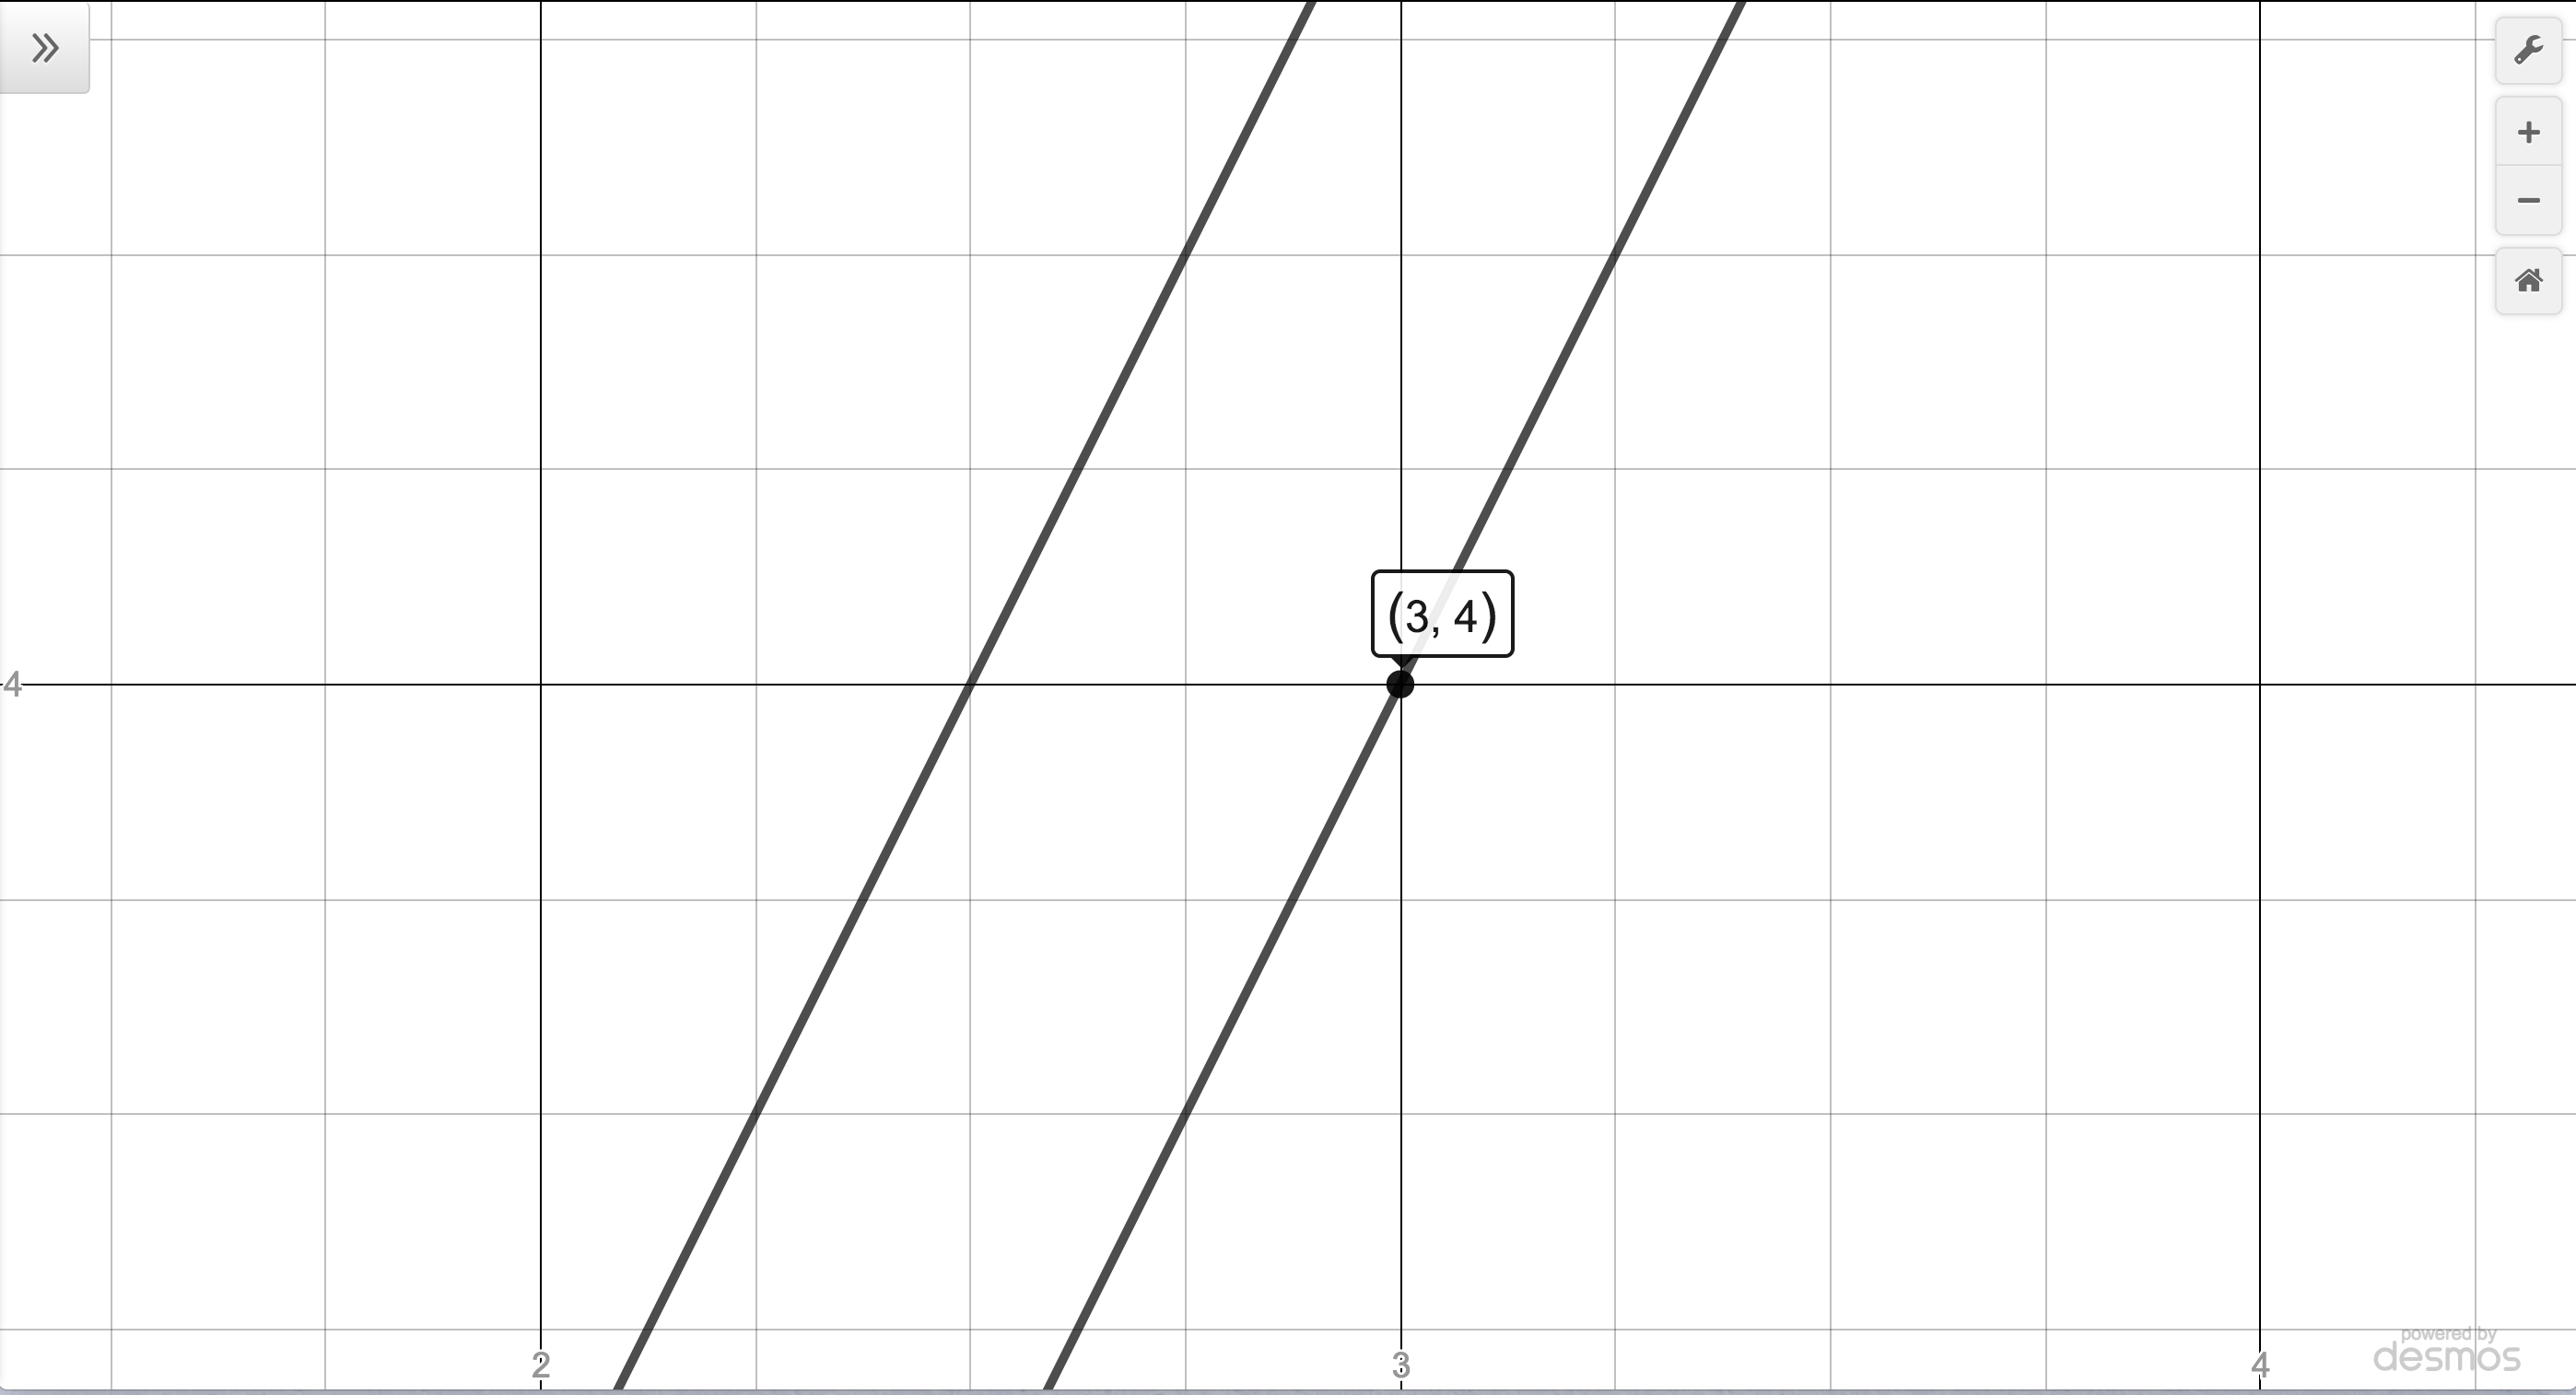
\includegraphics[width=2in]{./AppLinesGraphics/A5Graph01.jpg} &

\hspace{0.75in} 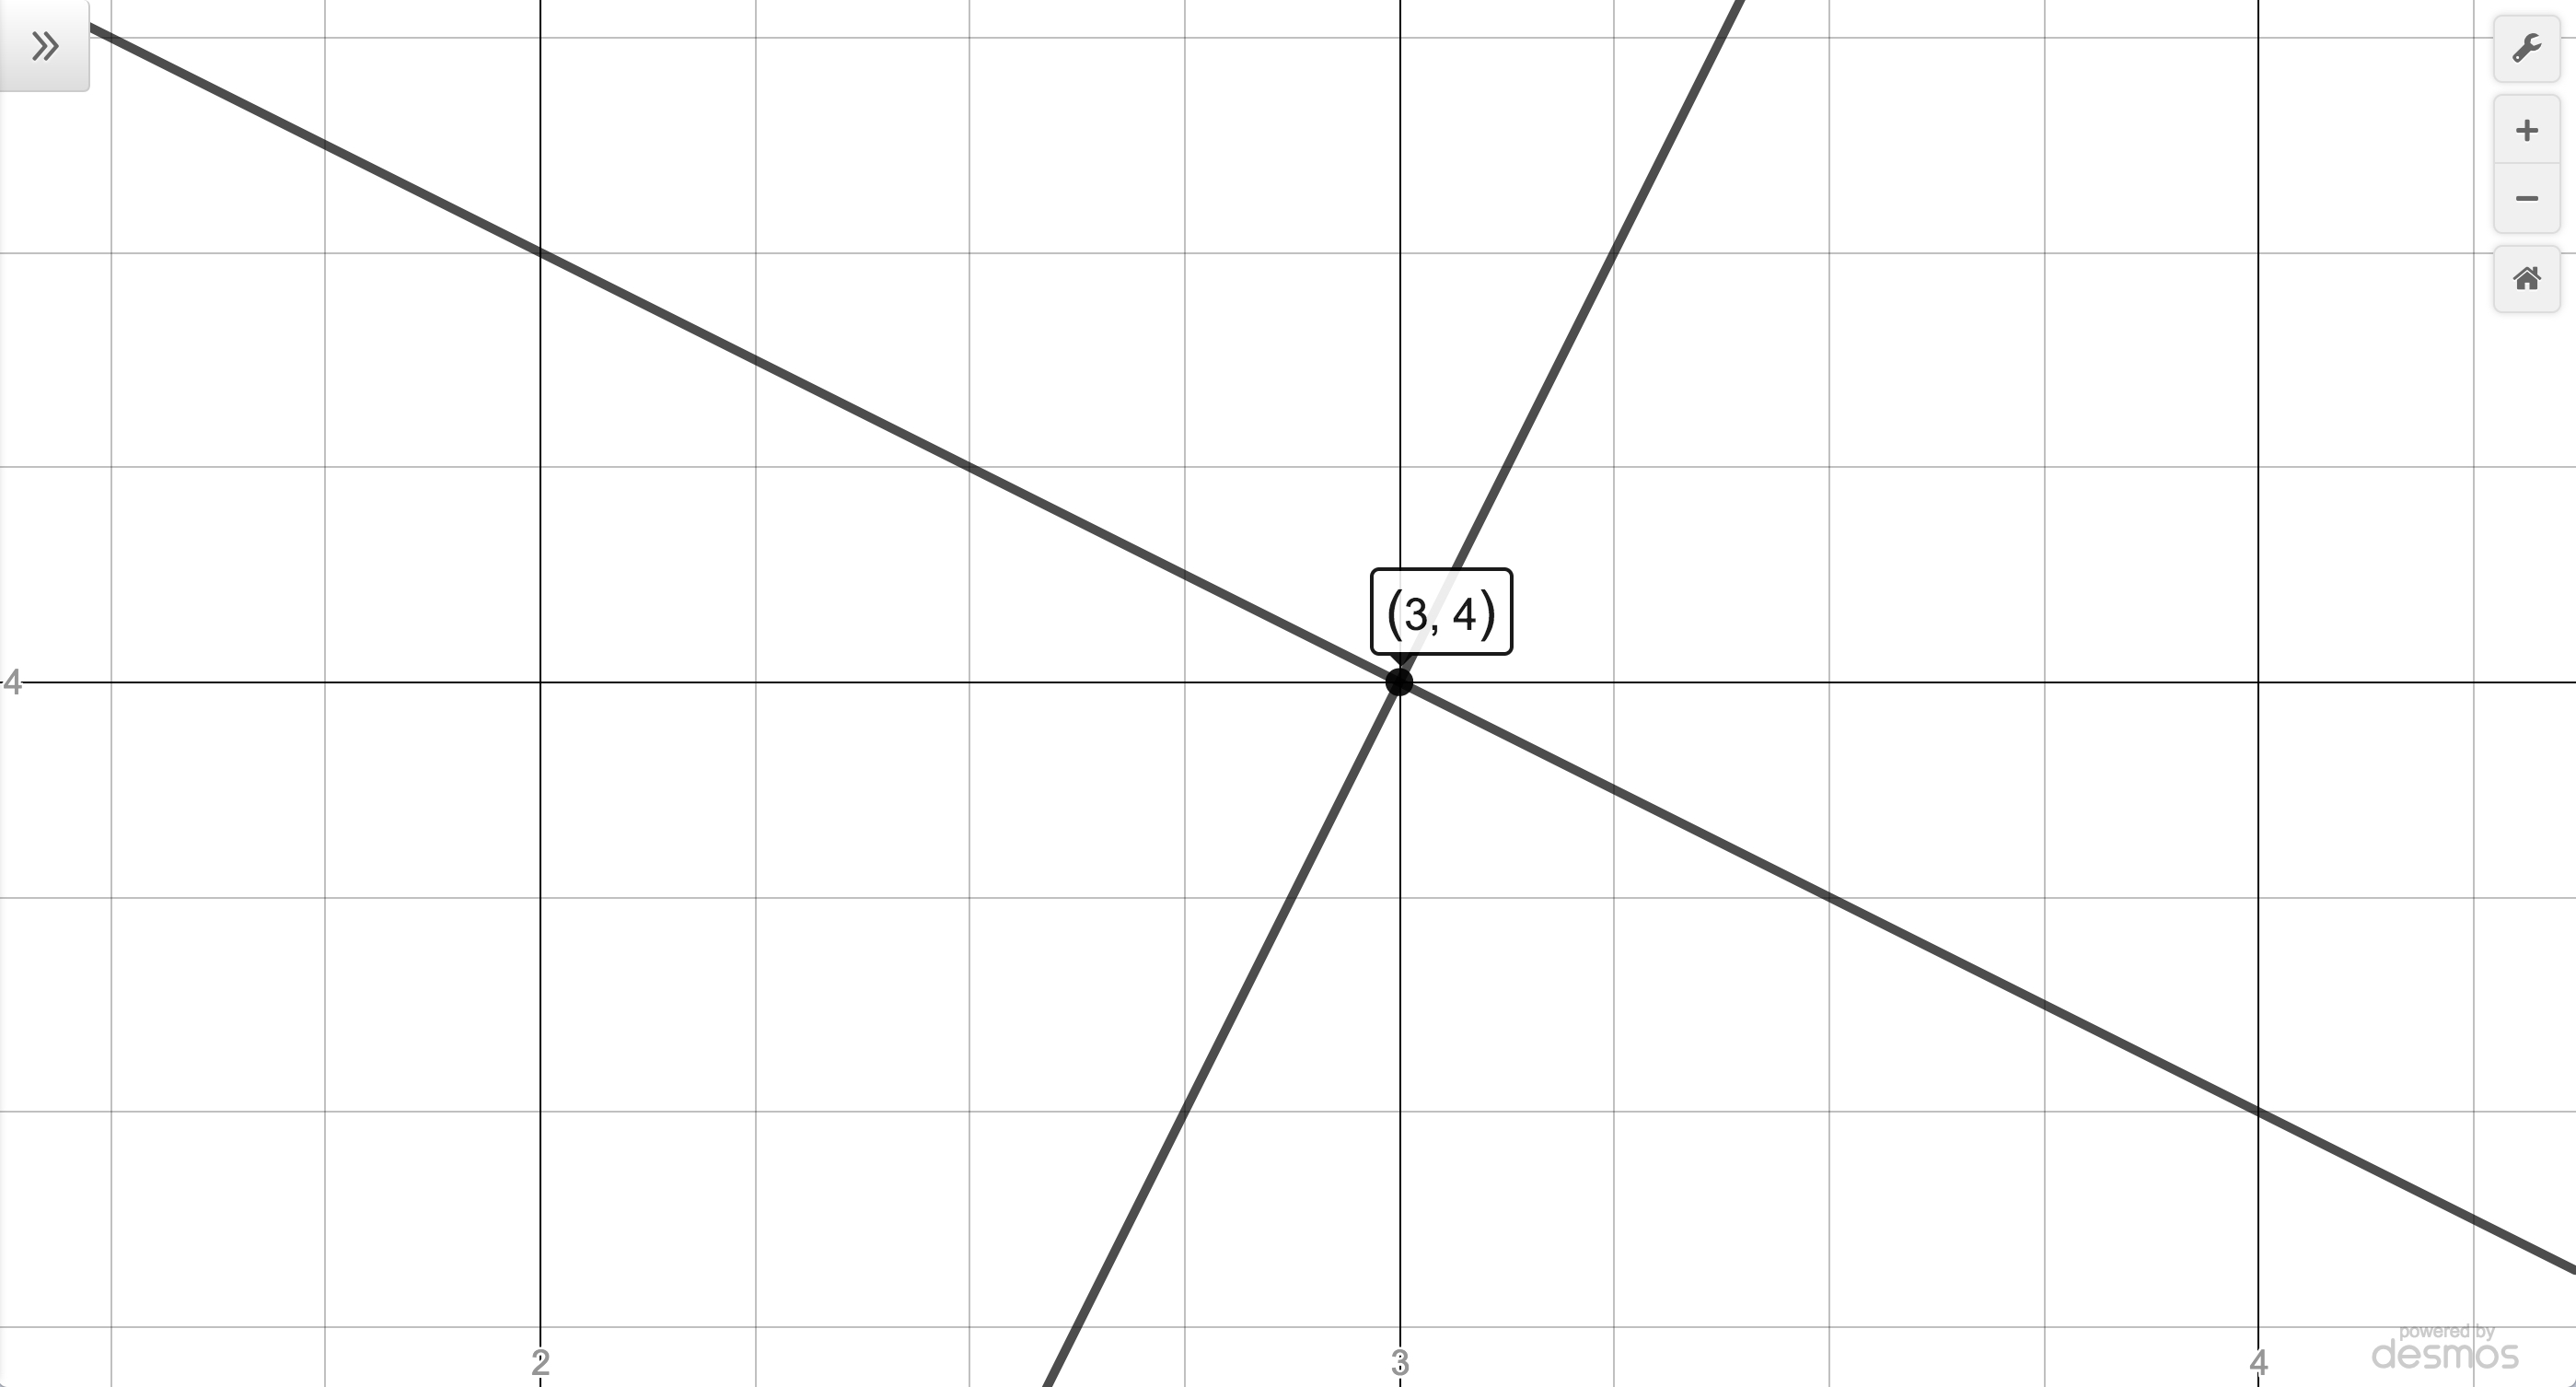
\includegraphics[width=2in]{./AppLinesGraphics/A5Graph02.jpg} \\

$y = 2x-1$ and  & 

 \hspace{0.75in}  $y = 2x-1$ and  \\
 
 \boldmath $y=2x-2$ & \hspace{0.75in} \boldmath $y= -\frac{1}{2} x + \frac{11}{2} $\\
 
\end{tabular}

\end{center}



\end{enumerate}


\end{ex}

\phantomsection

\label{inversemidpoint}

Our last example with lines sets up a fourth kind of symmetry which will be revisited in Section \ref{InverseFunctions}.  

\begin{ex} \label{inversemidpointex2} Show that the points $(a,b)$ and $(b,a)$ in the $xy$-plane are symmetric about the line $y = x$.  

\medskip

{\bf Solution.}  If $a = b$ then $(a, b) = (a, a) = (b, a)$ and this point lies on the line $y = x$.\footnote{Please ask your instructor if lying on the line counts as being `symmetric about the line' or not.}  To prove the claim for the case when $a \neq b$, we will show that the line $y = x$ is a perpendicular bisector of the line segment with endpoints $(a,b)$ and $(b,a)$, as illustrated below.


\begin{center}
\begin{mfpic}[15]{-1}{5}{-1}{5}
\arrow \reverse \arrow \polyline{(-1,-1), (4,4)}
\tlabel[cc](5,-0.5){\scriptsize $x$}
\tlabel[cc](0.5,5){\scriptsize $y$}
\tlabel[cc](1,3.5){\scriptsize $(a,b)$}
\tlabel[cc](3,0.5){\scriptsize $(b,a)$}
\dashed \polyline{(1,3), (3,1)}
\polyline{(2,2), (1.75, 2.25), (2,2.5), (2.25, 2.25)} 
\point[3pt]{(1,3),(3,1), (2,2)}
\tlpointsep{4pt}
\axes

\end{mfpic}


\end{center}



To show the `perpendicular' part,  we first note the slope of the line containing $(a,b)$ and $(b,a)$ is \[ m= \dfrac{a-b}{b-a} = \dfrac{\cancel{(a-b)}}{-\cancel{(b-a)}} = -1\]

Since the slope of $y = x = 1x + 0$ is $m = 1$,  we see that the slopes of these two lines are negative reciprocals.  Hence, $y=x$ and the line segment with endpoints $(a,b)$ and $(b,a)$ are perpendicular.  For the `bisector' part, we use Equation \ref{midpointformula} to find the midpoint of  the line segment with endpoints $(a,b)$ and $(b,a)$:

\setlength{\extrarowheight}{10pt}

\[ \begin{array}{rcl}

 M & = & \left( \dfrac{a+b}{2},  \dfrac{b+a}{2} \right) \\
   & = & \left( \dfrac{a+b}{2},  \dfrac{a+b}{2} \right)  \\ \end{array} \]

Since the $x$ and $y$ coordinates of this point are the same, we find that the midpoint lies on the line $y=x$. \qed

\end{ex}

\newpage

\subsection{Exercises}

\label{ExercisesforAppLines}

In Exercises \ref{pointslopegivenlinefirst} - \ref{pointslopegivenlinelast}, find both the point-slope form and the slope-intercept form of the line with the given slope which passes through the given point.

\begin{tasks}(2)
\task $m = 3, \;\; P(3, -1)$ \label{pointslopegivenlinefirst}
\task $m = -2, \;\; P(-5, 8)$
\task $m = -1, \;\; P(-7, -1)$
\task $m = \frac{2}{3}, \;\; P(-2, 1)$
\task $m = -\frac{1}{5}, \;\; P(10, 4)$
\task $m = \frac{1}{7}, \;\; P(-1, 4)$
\task $m = 0, \;\; P(3, 117)$
\task $m = -\sqrt{2}, \;\; P(0, -3)$
\task $m = -5, \;\; P(\sqrt{3}, 2\sqrt{3})$
\task $m = 678, \;\; P(-1, -12)$ \label{pointslopegivenlinelast}
\end{tasks}

In Exercises \ref{twopointsgivenlinefirst} - \ref{twopointsgivenlinelast}, find the slope-intercept form of the line which passes through the given points.

\begin{tasks}[resume](2)
\task $P(0, 0), \; Q(-3, 5)$ \label{twopointsgivenlinefirst}
\task $P(-1, -2), \; Q(3, -2)$
\task $P(5, 0), \; Q(0, -8)$
\task $P(3, -5), \; Q(7, 4)$
\task $P(-1,5), \; Q(7, 5)$
\task $P(4, -8), \; Q(5, -8)$
\task $P\left(\frac{1}{2}, \frac{3}{4} \right), \; Q\left(\frac{5}{2}, -\frac{7}{4} \right)$
\task $P\left(\frac{2}{3}, \frac{7}{2} \right), \; Q\left(-\frac{1}{3}, \frac{3}{2} \right)$
\task! $P\left(\sqrt{2}, -\sqrt{2} \right), \; Q\left(-\sqrt{2}, \sqrt{2} \right)$
\task $P\left(-\sqrt{3}, -1 \right), \; Q\left(\sqrt{3}, 1 \right)$ \label{twopointsgivenlinelast}
\end{tasks}

In Exercises \ref{graphlineexerfirst} - \ref{graphlineexerlast}, graph the line.  Find the slope, $y$-intercept and $x$-intercept, if any exist.

\begin{tasks}[resume](2)
\task $y = 2x - 1$ \label{graphlineexerfirst}
\task $y = 3 - x$
\task $y = 3$
\task $y = 0$
\task $y = \frac{2}{3} x + \frac{1}{3}$ \vphantom{$\dfrac{1-x}{2}$}
\task $y = \dfrac{1-x}{2}$ \label{graphlineexerlast}
\task!  Graph $3v + 2w = 6$ on both the $vw$- and $wv$-axes.  What characteristics to both graphs share?  What's different?
\task!  Find all of the points on the line $y=2x+1$ which are $4$ units from the point $(-1,3)$.
\end{tasks}

In Exercises \ref{parallelfirst} - \ref{parallellast}, you are given a line and a point which is not on that line.  Find the line parallel to the given line which passes through the given point.

\begin{tasks}[resume](2)
\task $y = 3x + 2, \; P(0, 0)$ \label{parallelfirst}
\task $y = -6x + 5, \; P(3, 2)$
\task $y = \frac{2}{3} x - 7, \; P(6, 0)$
\task $y = \dfrac{4-x}{3}, \; P(1, -1)$
\task $y = 6, \; P(3, -2)$
\task $x=1, \; P(-5,0)$ \label{parallellast}
\end{tasks}

\phantomsection
\label{perpendicularlines}

In Exercises \ref{perpendlinefirst} - \ref{perpendlinelast}, you are given a line and a point which is not on that line.  Find the line perpendicular to the given line which passes through the given point.

\begin{tasks}[resume](2)
\task $y = \frac{1}{3}x + 2, \; P(0, 0)$ \label{perpendlinefirst}
\task $y = -6x + 5, \; P(3, 2)$
\task $y = \frac{2}{3} x - 7, \; P(6, 0)$
\task $y = \dfrac{4-x}{3}, \; P(1, -1)$
\task $y = 6, \; P(3, -2)$
\task $x=1, \; P(-5,0)$ \label{perpendlinelast}
\task! We shall now prove that $y = m_{\mbox{\tiny$1$}}x + b_{\mbox{\tiny$1$}}$ is perpendicular to $y = m_{\mbox{\tiny$2$}}x + b_{\mbox{\tiny$2$}}$ if and only if $m_{\mbox{\tiny$1$}} \cdot m_{\mbox{\tiny$2$}} = -1$.  To make our lives easier we shall assume that $m_{\mbox{\tiny$1$}} > 0$ and $m_{\mbox{\tiny$2$}} < 0$.  We can also ``move'' the lines so that their point of intersection is the origin without messing things up, so we'll assume $b_{\mbox{\tiny$1$}} = b_{\mbox{\tiny$2$}} = 0.$  (Take a moment with your classmates to discuss why this is okay.)  Graphing the lines and plotting the points $O(0, 0)\;$, $P(1, m_{\mbox{\tiny$1$}})\;$ and $Q(1, m_{\mbox{\tiny$2$}})$ gives us the following set up. \label{perpendicularlineproof}

\begin{center}

\begin{mfpic}[18]{-5}{5}{-5}{5}
\point[3pt]{(0, 0), (1.5, 0.75), (1.5, -3)}
\arrow \reverse \arrow \polyline{( -4, -2), (4, 2)}
\arrow \reverse \arrow \polyline{( -2, 4), (2, -4)}
\polyline{(1.5, 0.75), (1.5, -3)}
\tlabel(1.2, 1){\scriptsize $P$}
\tlabel(-.5,-.6){\scriptsize $O$}
\tlabel(1.2,-3.55){\scriptsize $Q$}
\axes
\tlabel[cc](5,-0.5){\scriptsize $x$}
\tlabel[cc](0.5,5){\scriptsize $y$}
\end{mfpic}

\end{center}

The line $y = m_{\mbox{\tiny$1$}}x$ will be perpendicular to the line $y = m_{\mbox{\tiny$2$}}x$ if and only if $\bigtriangleup OPQ$ is a right triangle.  Let $d_{\mbox{\tiny$1$}}$ be the distance from $O$ to $P$, let $d_{\mbox{\tiny$2$}}$ be the distance from $O$ to $Q$ and let $d_{\mbox{\tiny$3$}}$ be the distance from $P$ to $Q$.  Use the Pythagorean Theorem to show that $\bigtriangleup OPQ$ is a right triangle if and only if $m_{\mbox{\tiny$1$}} \cdot m_{\mbox{\tiny$2$}} = -1$ by showing $d_{\mbox{\tiny$1$}}^{2} + d_{\mbox{\tiny$2$}}^{2} = d_{\mbox{\tiny$3$}}^2$ if and only if $m_{\mbox{\tiny$1$}} \cdot m_{\mbox{\tiny$2$}} = -1$.  
\end{tasks}

\newpage

\subsection{Answers}

\begin{tasks}(2)
\task $y+1 = 3(x-3)$ \\ $y = 3x-10$
\task $y-8 = -2(x+5)$ \\ $y = -2x-2$
\task $y + 1 = -(x+7)$ \\ $y = -x-8$
\task $y - 1 = \frac{2}{3} (x+2)$ \\ $y = \frac{2}{3} x + \frac{7}{3}$
\task $y - 4 = -\frac{1}{5} (x-10)$ \\ $y = -\frac{1}{5} x + 6$
\task $y - 4 = \frac{1}{7}(x + 1)$ \\ $y = \frac{1}{7}x + \frac{29}{7}$
\task $y - 117 = 0$ \\ $y = 117$
\task $y + 3 = -\sqrt{2}(x - 0)$ \\ $y = -\sqrt{2}x - 3$
\task $y - 2\sqrt{3} = -5(x - \sqrt{3})$ \\ $y = -5x + 7\sqrt{3}$ 
\task $y + 12 = 678(x + 1)$ \\ $y = 678x + 666$
\task $y = -\frac{5}{3}x$
\task $y = -2$
\task $y = \frac{8}{5}x - 8$ 
\task $y = \frac{9}{4}x - \frac{47}{4}$
\task $y = 5$
\task $y = -8$
\task $y = -\frac{5}{4} x + \frac{11}{8}$ 
\task $y = 2x + \frac{13}{6}$ 
\task $y = -x$
\task $y = \frac{\sqrt{3}}{3} x$
\task! \begin{multicols}{2} \raggedcolumns
$y =2x-1$

slope: $m = 2$ 

$y$-intercept:  $(0,-1)$

$x$-intercept: $\left(\frac{1}{2}, 0 \right)$
\columnbreak
\begin{mfpic}[15]{-3}{3}{-4}{4}
\point[3pt]{(0,-1), (0.5,0)}
\axes
\tlabel[cc](3,-0.5){\scriptsize $x$}
\tlabel[cc](0.5,4){\scriptsize $y$}
\xmarks{-2,-1,1,2}
\ymarks{-3,-2,-1,1,2,3}
\tlpointsep{4pt}
\tiny 
\axislabels {x}{{$-2 \hspace{6pt}$} -2,{$-1 \hspace{6pt}$} -1, {$1$} 1, {$2$} 2}
\axislabels {y}{{$-3$} -3,{$-2$} -2,{$-1$} -1, {$1$} 1, {$2$} 2, {$3$} 3}
\normalsize
\arrow \reverse \arrow \function{-1,2, 0.1}{2*x-1}
\end{mfpic} 
\end{multicols}

\task! \begin{multicols}{2} \raggedcolumns
$y =3-x$

slope: $m = -1$ 

$y$-intercept:  $(0,3)$

$x$-intercept: $(3, 0)$ 

\columnbreak

\begin{mfpic}[15]{-2}{5}{-2}{5}
\point[3pt]{(0,3), (3,0)}
\axes
\tlabel[cc](5,-0.5){\scriptsize $x$}
\tlabel[cc](0.5,5){\scriptsize $y$}
\xmarks{-1,1,2,3,4}
\ymarks{-1,1,2,3,4}
\tlpointsep{4pt}
\tiny 
\axislabels {x}{{$-1 \hspace{6pt}$} -1, {$1$} 1, {$2$} 2, {$3$} 3, {$4$} 4}
\axislabels {y}{{$-1$} -1, {$1$} 1, {$2$} 2, {$3$} 3, {$4$} 4}
\normalsize
\arrow \reverse \arrow \function{-1,4, 0.1}{3-x}
\end{mfpic}
\end{multicols}

\task! \begin{multicols}{2} \raggedcolumns
$y = 3$

slope: $m =0$ 

$y$-intercept:  $(0,3)$

$x$-intercept: none

\columnbreak
\begin{mfpic}[15]{-3}{3}{-1}{5}
\point[3pt]{(0,3)}
\axes
\tlabel[cc](3,-0.5){\scriptsize $x$}
\tlabel[cc](0.5,5){\scriptsize $y$}
\xmarks{-2,-1,1,2}
\ymarks{1,2,3,4}
\tlpointsep{4pt}
\tiny 
\axislabels {x}{{$-2 \hspace{6pt}$} -2,{$-1 \hspace{6pt}$} -1, {$1$} 1, {$2$} 2}
\axislabels {y}{{$1$} 1, {$2$} 2, {$3$} 3, {$4$} 4}
\normalsize
\arrow \reverse \arrow \function{-3,3, 0.1}{3}
\end{mfpic}
\end{multicols}

\task! \begin{multicols}{2} \raggedcolumns
$y = 0$

slope: $m =0$ 

$y$-intercept:  $(0,0)$

$x$-intercept:

$\{ (x,0) \, | \, \text{$x$ is a real number} \}$

\columnbreak
\begin{mfpic}[15]{-3}{3}{-2}{2}
\arrow \polyline{(0,-2), (0,2)}
\tlabel[cc](3,-0.5){\scriptsize $x$}
\tlabel[cc](0.5,2){\scriptsize $y$}
\xmarks{-2,-1,1,2}
\ymarks{-1,1}
\tlpointsep{4pt}
\tiny 
\axislabels {x}{{$-2 \hspace{6pt}$} -2,{$-1 \hspace{6pt}$} -1, {$1$} 1, {$2$} 2}
\axislabels {y}{{$-1$} -1,{$1$} 1}
\normalsize
\penwd{1.15pt}
\arrow \reverse \arrow \function{-3,3, 0.1}{0}
\end{mfpic}
\end{multicols}

\task! \begin{multicols}{2} \raggedcolumns
$y = \frac{2}{3} x + \frac{1}{3}$

slope: $m = \frac{2}{3}$ 

$y$-intercept:  $\left(0, \frac{1}{3}\right)$

$x$-intercept:  $\left(-\frac{1}{2}, 0\right)$

\columnbreak
\begin{mfpic}[15]{-3}{3}{-2}{3}
\point[3pt]{(0,0.33333), (-0.5,0)}
\axes
\tlabel[cc](3,-0.5){\scriptsize $x$}
\tlabel[cc](0.5,3){\scriptsize $y$}
\xmarks{-2,-1,1,2}
\ymarks{-1,1,2}
\tlpointsep{4pt}
\tiny 
\axislabels {x}{{$-2 \hspace{6pt}$} -2, {$1$} 1, {$2$} 2}
\axislabels {y}{{$-1$} -1, {$1$} 1, {$2$} 2}
\normalsize
\arrow \reverse \arrow \function{-3,3, 0.1}{0.66667*x+0.33333}
\end{mfpic}
\end{multicols}

\task! \begin{multicols}{2} \raggedcolumns
$y = \dfrac{1-x}{2}$

slope: $m = -\frac{1}{2}$ 

$y$-intercept:  $\left(0, \frac{1}{2}\right)$

$x$-intercept:  $\left(1, 0\right)$

\columnbreak
\begin{mfpic}[15]{-3}{3}{-2}{3}
\point[3pt]{(0,0.5), (1,0)}
\axes
\tlabel[cc](3,-0.5){\scriptsize $x$}
\tlabel[cc](0.5,3){\scriptsize $y$}
\xmarks{-2,-1,1,2}
\ymarks{-1,1,2}
\tlpointsep{4pt}
\tiny 
\axislabels {x}{{$-2 \hspace{6pt}$} -2,{$-1 \hspace{6pt}$} -1, {$1$} 1, {$2$} 2}
\axislabels {y}{{$-1$} -1, {$1$} 1, {$2$} 2}
\normalsize
\arrow \reverse \arrow \function{-3,3, 0.1}{0.5-0.5*x}
\end{mfpic}
\end{multicols}

\task! \begin{multicols}{2} \raggedcolumns
$w = -\frac{3}{2} v + 3$

slope: $m = -\frac{3}{2}$ 

$w$-intercept:  $\left(0, 3\right)$

$v$-intercept:  $\left(2, 0\right)$

\columnbreak
\begin{mfpic}[15]{-1}{4}{-1}{4}
\point[3pt]{(0,3), (2,0)}
\axes
\tlabel[cc](4,-0.5){\scriptsize $v$}
\tlabel[cc](0.5,4){\scriptsize $w$}
\xmarks{1,2,3}
\ymarks{1,2,3}
\tlpointsep{4pt}
\tiny 
\axislabels {x}{{$1$} 1, {$2$} 2, {$3$} 3}
\axislabels {y}{{$1$} 1, {$2$} 2, , {$3$} 3}
\normalsize
\arrow \reverse \arrow \polyline{(-0.5, 3.75), (2.5, -0.75)}
\end{mfpic}
\end{multicols}

\begin{multicols}{2} \raggedcolumns
$v = -\frac{2}{3} w + 2$

slope: $m = -\frac{2}{3}$ 

$v$-intercept:  $\left(0,2 \right)$

$w$-intercept:  $\left(3,0\right)$

\columnbreak
\begin{mfpic}[15]{-1}{4}{-1}{4}
\point[3pt]{(0,2), (3,0)}
\axes
\tlabel[cc](4,-0.5){\scriptsize $w$}
\tlabel[cc](0.5,4){\scriptsize $v$}
\xmarks{1,2,3}
\ymarks{1,2,3}
\tlpointsep{4pt}
\tiny 
\axislabels {x}{{$1$} 1, {$2$} 2, {$3$} 3}
\axislabels {y}{{$1$} 1, {$2$} 2, , {$3$} 3}
\normalsize
\arrow \reverse \arrow \polyline{(3.75, -0.5), (-0.75, 2.5)}
\end{mfpic}
\end{multicols} 

\task $(-1,-1)$ and $\left(\frac{11}{5}, \frac{27}{5}\right)$
\task $y = 3x$
\task $y = -6x + 20$
\task $y = \frac{2}{3} x - 4$
\task $y = -\frac{1}{3} x - \frac{2}{3}$
\task $y=-2$
\task $x=-5$
\task $y = -3x$
\task $y = \frac{1}{6}x + \frac{3}{2}$
\task $y = -\frac{3}{2} x +9$
\task $y = 3x-4$
\task $x=3$
\task $y=0$
\end{tasks}

\closegraphsfile